\documentclass[11pt]{article}

\usepackage[T1]{fontenc}
\usepackage{lmodern}
\usepackage{microtype}
\usepackage[margin=1in]{geometry}
\usepackage{amsmath,amssymb,amsthm,mathtools}
\usepackage{bm}
\usepackage{xcolor}
\usepackage{enumitem}
\usepackage{booktabs,tabularx,array}
\usepackage{tikz}
\usetikzlibrary{arrows.meta,positioning,calc,fit}
\usepackage[most]{tcolorbox}
\usepackage{fancyhdr}
\usepackage{hyperref}
\usepackage{needspace}

\definecolor{navy}{HTML}{17365D}
\definecolor{teal}{HTML}{147D92}
\definecolor{blueback}{HTML}{EEF5FA}
\definecolor{greenback}{HTML}{EEF7F2}
\definecolor{greenframe}{HTML}{39735B}
\definecolor{amberback}{HTML}{FFF7E8}
\definecolor{amberframe}{HTML}{A66A14}
\definecolor{grayback}{HTML}{F5F6F8}
\definecolor{darkgray}{HTML}{3B4048}
\definecolor{roseback}{HTML}{FFF1F1}
\definecolor{roseframe}{HTML}{985050}

\hypersetup{
  colorlinks=true,
  linkcolor=navy,
  citecolor=teal,
  urlcolor=teal,
  pdftitle={A Research Program for Conditional Mutual Information and Quantum Markov Recovery in CFT},
  pdfauthor={Technical research note}
}

\pagestyle{fancy}
\fancyhf{}
\fancyhead[L]{\small\color{darkgray}Conditional mutual information in CFT}
\fancyhead[R]{\small\color{darkgray}Research program}
\fancyfoot[C]{\small\thepage}
\renewcommand{\headrulewidth}{0.4pt}
\setlength{\headheight}{14pt}

\newtheoremstyle{accenttheorem}
  {8pt}{8pt}{\itshape}{}
  {\color{navy}\bfseries}{.}{0.5em}{}
\theoremstyle{accenttheorem}
\newtheorem{conjecture}{Conjecture}
\newtheorem{problem}[conjecture]{Problem}
\newtheorem{target}[conjecture]{Target theorem}

\theoremstyle{definition}
\newtheorem{definition}[conjecture]{Definition}
\newtheorem{remark}[conjecture]{Remark}

\newcommand{\cA}{\mathcal{A}}
\newcommand{\cR}{\mathcal{R}}
\newcommand{\cE}{\mathcal{E}}
\newcommand{\cH}{\mathcal{H}}
\newcommand{\cM}{\mathfrak{M}}
\newcommand{\cN}{\mathfrak{N}}
\newcommand{\cQ}{\mathfrak{Q}}
\newcommand{\id}{\operatorname{id}}
\newcommand{\Tr}{\operatorname{Tr}}
\newcommand{\CMI}{I}
\newcommand{\MI}{F}
\newcommand{\RE}{D}
\newcommand{\eps}{\varepsilon}
\newcommand{\dd}{\,\mathrm{d}}
\newcommand{\1}{\mathbf{1}}
\newcommand{\supp}{\operatorname{supp}}
\newcommand{\Ad}{\operatorname{Ad}}
\newcommand{\CAR}{\operatorname{CAR}}
\newcommand{\Schatten}{\mathcal{S}}

\newtcolorbox{mainbox}[1][]{
  enhanced,
  colback=blueback,
  colframe=navy,
  boxrule=0.8pt,
  arc=2mm,
  left=5mm,right=5mm,top=3.5mm,bottom=3.5mm,
  title={\bfseries Research thesis},
  coltitle=white,
  colbacktitle=navy,
  attach boxed title to top left={xshift=4mm,yshift=-2mm},
  #1
}

\newtcolorbox{establishedbox}[1][]{
  enhanced,
  colback=greenback,
  colframe=greenframe,
  boxrule=0.7pt,
  arc=1.8mm,
  left=4.5mm,right=4.5mm,top=3mm,bottom=3mm,
  title={\bfseries Established input},
  coltitle=white,
  colbacktitle=greenframe,
  #1
}

\newtcolorbox{conjecturebox}[1][]{
  enhanced,
  colback=amberback,
  colframe=amberframe,
  boxrule=0.7pt,
  arc=1.8mm,
  left=4.5mm,right=4.5mm,top=3mm,bottom=3mm,
  title={\bfseries Proposed direction},
  coltitle=white,
  colbacktitle=amberframe,
  #1
}

\newtcolorbox{caveatbox}[1][]{
  enhanced,
  colback=grayback,
  colframe=darkgray!65,
  boxrule=0.65pt,
  arc=1.5mm,
  left=4.5mm,right=4.5mm,top=3mm,bottom=3mm,
  title={\bfseries Technical caveat},
  coltitle=darkgray,
  colbacktitle=grayback,
  #1
}

\newtcolorbox{highriskbox}[1][]{
  enhanced,
  colback=roseback,
  colframe=roseframe,
  boxrule=0.65pt,
  arc=1.5mm,
  left=4.5mm,right=4.5mm,top=3mm,bottom=3mm,
  title={\bfseries High-risk / high-payoff idea},
  coltitle=white,
  colbacktitle=roseframe,
  #1
}

\setlist[itemize]{leftmargin=1.5em,itemsep=2.5pt,topsep=4pt}
\setlist[enumerate]{leftmargin=1.7em,itemsep=3pt,topsep=4pt}
\setlength{\parindent}{0pt}
\setlength{\parskip}{5.5pt}
\allowdisplaybreaks
\emergencystretch=2em

\title{\vspace{-1.5cm}\color{navy}\bfseries
A Research Program for Conditional Mutual Information\newline
and Quantum Markov Recovery in Conformal Field Theory\\[0.4em]
\large From Longo--Xu finiteness to continuum Petz maps, RG diagnostics, and Markov networks}
\author{}
\date{}

\begin{document}
\maketitle
\vspace{-1.5em}

\begin{abstract}
Longo and Xu give a rigorous, finite conditional mutual information for three adjacent intervals in an important class of chiral conformal nets.  Petz sufficiency and modern recovery theorems identify this quantity as a defect of quantum Markov reconstruction.  This note develops a concrete research program around that bridge.  The conceptual priority is to construct a recovery channel directly at zero collar width in type-III algebraic quantum field theory.  The most tractable entry point is the free chiral fermion, where Longo--Xu singular-integral methods can be combined with explicit fermionic Gaussian Petz maps.  Further directions include sharper CFT-specific recovery inequalities, a classification of exact geometric Markov configurations, an RG-scale ``Markov c-function,'' thermal/KMS states, superselection-sector sensitivity, multi-interval recovery networks, and extensions beyond the free-fermion finite-index class.  Throughout, established results are separated from conjectural targets and technical risks.
\end{abstract}

\begin{mainbox}
The most natural organizing principle is
\[
\boxed{
\begin{gathered}
\text{finite CFT CMI}
 = \text{finite loss of Araki relative entropy}\\[-1mm]
 = \text{quantitative obstruction to local recovery}
\end{gathered}}
\]
The most focused first project is to solve continuum Petz recovery for the free chiral fermion.  The larger structural goal is to decide whether the collar-regularized recovery maps converge to a single normal channel on the touching interval algebra, or whether the correct continuum object is intrinsically an asymptotic recovery net.
\end{mainbox}

\vspace{0.6em}
\begin{center}
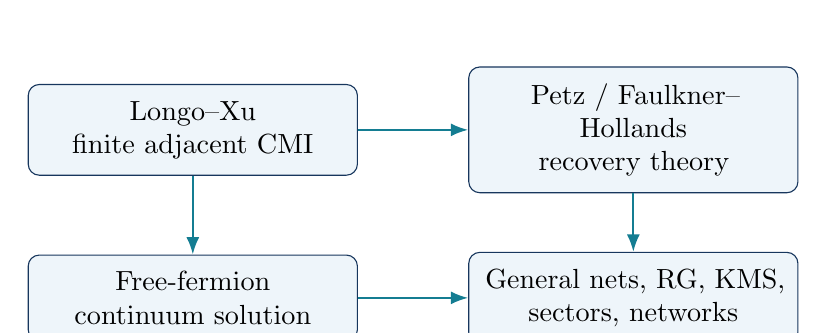
\begin{tikzpicture}[
  node distance=10mm and 14mm,
  box/.style={draw=navy,rounded corners,fill=blueback,align=center,inner sep=6pt,text width=0.31\textwidth},
  arr/.style={-{Latex[length=2.2mm]},thick,draw=teal}
]
\node[box] (lx) {Longo--Xu\\finite adjacent CMI};
\node[box,right=of lx] (fh) {Petz / Faulkner--Hollands\\recovery theory};
\node[box,below=of lx] (ff) {Free-fermion\\continuum solution};
\node[box,right=of ff] (gen) {General nets, RG, KMS,\\sectors, networks};
\draw[arr] (lx) -- (fh);
\draw[arr] (lx) -- (ff);
\draw[arr] (fh) -- (gen);
\draw[arr] (ff) -- (gen);
\end{tikzpicture}
\end{center}

\clearpage
\tableofcontents
\clearpage

\section{Established starting point}

Let
\[
 A=(x_0,x_1),\qquad B=(x_1,x_2),\qquad C=(x_2,x_3),
 \qquad x_0<x_1<x_2<x_3,
\]
and set
\[
 a=x_1-x_0,\qquad b=x_2-x_1,\qquad c=x_3-x_2.
\]
It is useful to adopt the cross-ratio convention
\begin{equation}\label{eq:x-def}
 x:=\frac{ac}{(a+b)(b+c)},
 \qquad
 1-x=\frac{b(a+b+c)}{(a+b)(b+c)}.
\end{equation}
Thus shielding by a long middle interval corresponds to \(x\downarrow0\).

For the free chiral fermion net in the normalization used by Longo and Xu, and for the finite-index class controlled by their methods, the adjacent-interval conditional mutual information is
\begin{equation}\label{eq:longo-xu-cmi}
 \CMI_\omega(A:C\mid B)
 =\kappa\log\frac{(a+b)(b+c)}{b(a+b+c)}
 =-\kappa\log(1-x),
\end{equation}
with \(\kappa=r/6\) for their \(r\)-component free-fermion normalization \cite{LongoXu}.  For a full parity-symmetric \(1+1\)-dimensional CFT vacuum, the usual entropy normalization gives \(\kappa=c/3\).

The formula is finite and positive for \(a,b,c>0\).  In particular,
\begin{equation}\label{eq:large-b-cmi}
 \CMI_\omega(A:C\mid B)
 =\kappa\frac{ac}{b^2}+O(b^{-3})
 \qquad (b\gg a+c).
\end{equation}

To connect this with recovery, introduce a collar
\[
 A_\eps=(x_0,x_1-\eps),\qquad \eps>0,
\]
and the inclusions
\begin{equation}\label{eq:collar-inclusion}
 \cN_\eps
 :=\cA(A_\eps)\vee\cA(B)
 \subset
 \cM_\eps
 :=\cA(A_\eps)\vee\cA(BC).
\end{equation}
The split property produces the normal product reference state
\[
 \sigma_\eps=\omega_{A_\eps}\otimes\omega_{BC}
\]
on \(\cM_\eps\).  Longo--Xu's chain rule identifies the regulated CMI with a relative-entropy loss:
\begin{equation}\label{eq:dpi-defect}
 \CMI_\eps(A:C\mid B)
 =\RE_{\cM_\eps}(\omega\Vert\sigma_\eps)
 -\RE_{\cN_\eps}
 \bigl(\omega|_{\cN_\eps}\Vert\sigma_\eps|_{\cN_\eps}\bigr).
\end{equation}
The singular pieces of the two terms cancel as \(\eps\downarrow0\), and the limit is \eqref{eq:longo-xu-cmi}.

Petz's equality theorem says that vanishing loss of relative entropy is equivalent to exact recoverability \cite{Petz1986,Petz1988}.  The finite-dimensional equality states are precisely short quantum Markov chains in the sense of Hayden--Jozsa--Petz--Winter \cite{HJPW}.  Fawzi--Renner and the universal recovery results of Junge--Renner--Sutter--Wilde--Winter quantify the approximate case \cite{FawziRenner,JungeEtAl}.  Faulkner--Hollands--Swingle--Wang extend the relevant strengthened data-processing statement to arbitrary von Neumann subalgebras \cite{FaulknerEtAl}.

At every fixed \(\eps>0\), one therefore obtains a normal recovery channel and a recovered state \(\widetilde\omega_\eps\) satisfying schematically
\begin{equation}\label{eq:fh-bound}
 \CMI_\eps(A:C\mid B)
 \ge -2\log F(\omega,\widetilde\omega_\eps).
\end{equation}
Consequently,
\begin{equation}\label{eq:liminf-recovery}
 \liminf_{\eps\downarrow0}F(\omega,\widetilde\omega_\eps)
 \ge \exp\!\left[-\frac12\CMI_\omega(A:C\mid B)\right]
 =(1-x)^{\kappa/2}.
\end{equation}

\begin{establishedbox}
Equations \eqref{eq:longo-xu-cmi}--\eqref{eq:liminf-recovery} already provide an operational statement: the cross ratio controls a universal lower bound on how well the vacuum can be reconstructed from \(AB\) by acting only through the middle region.  What is not yet automatic is the existence of a single normal recovery channel after the collar has been removed.
\end{establishedbox}

\section{The central continuum problem: remove the collar}

The conceptual next step is to replace the family of regulated recovery statements by a recovery statement intrinsic to the touching type-III algebras.

In the Heisenberg picture, let
\[
 \alpha_\eps:\cM_\eps\longrightarrow\cN_\eps
\]
be a Petz or modularly averaged Petz map associated with the pair \((\sigma_\eps,\cN_\eps\subset\cM_\eps)\).  Its dual reconstructs a state on \(\cM_\eps\) from its restriction to \(\cN_\eps\).  The natural zero-collar target is a normal unital completely positive map
\begin{equation}\label{eq:alpha0}
 \alpha_0:\cA(ABC)\longrightarrow\cA(AB)
\end{equation}
whose dual acts as a continuum recovery channel \(AB\to ABC\).

\begin{target}[Zero-collar recovery]
Assume a strongly additive split conformal net in the Longo--Xu class.  Prove that an appropriate choice of regulated recovery maps has a locally normal limit \(\alpha_0\) as in \eqref{eq:alpha0}, and that the recovered state obeys
\[
 F\bigl(\omega,\omega|_{\cA(AB)}\circ\alpha_0\bigr)
 \ge (1-x)^{\kappa/2}.
\]
A weaker but still valuable theorem would construct a recovery map on the quasilocal \(C^*\)-algebra and then identify conditions ensuring normal extension to \(\cA(ABC)\).
\end{target}

The split factorization at \(\eps>0\) suggests that the nontrivial part of the channel should depend only on
\[
 \cA(B)\subset\cA(BC)
\]
and the vacuum on \(BC\).  Formally one would like
\begin{equation}\label{eq:formal-localized-map}
 \alpha_0\bigl(X_A Y_{BC}\bigr)
 =X_A\,\alpha_{BC\to B}(Y_{BC}),
 \qquad
 X_A\in\cA(A),\quad Y_{BC}\in\cA(BC).
\end{equation}
The problem is not the algebraic formula; it is proving that it extends boundedly, completely positively, and normally through the non-split touching boundary.

\subsection{A useful hierarchy of limiting statements}

Rather than attacking normal convergence in one step, it is useful to separate four increasingly strong goals.

\begin{enumerate}
\item \textbf{Local observable convergence.}  For each interval \(A'\Subset A\), prove convergence on
\[
 \cA(A')\vee\cA(BC),
\]
where a positive separation remains.

\item \textbf{Quasilocal \(C^*\)-limit.}  Show that the compatible local limits define a completely positive map on the inductive-limit algebra generated by compactly contained intervals.

\item \textbf{Locally normal recovered state.}  Prove that the states
\[
 \widetilde\omega_\eps
 =\omega|_{\cN_\eps}\circ\alpha_\eps
\]
converge on every fixed local algebra to a locally normal state.

\item \textbf{Normal channel on the touching factor.}  Establish point-ultraweak convergence, or another normal extension criterion, producing \eqref{eq:alpha0}.
\end{enumerate}

Potential tools include hyperfiniteness or injectivity of local factors, compactness of normal completely positive maps in suitable weak topologies, modular nuclearity, energy bounds, and direct estimates on Connes cocycles.  The key point is that none of these tools by itself guarantees preservation of the desired localization and reference-state properties.

\begin{caveatbox}
There may be no single normal map satisfying all desired locality properties.  A negative theorem would still be structurally important: it would show that continuum quantum Markov recovery at a sharp boundary is correctly described by an asymptotic net \(\{\alpha_\eps\}_{\eps>0}\), not by one channel.  The distinction is invisible in a lattice regularization but potentially intrinsic to type-III locality.
\end{caveatbox}

\subsection{Approximate commuting squares}

The interval algebras form the geometric square
\[
\begin{matrix}
 \cA(B) &\subset& \cA(AB)\\[1mm]
 \cap && \cap\\[1mm]
 \cA(BC)&\subset&\cA(ABC).
\end{matrix}
\]
For an exact Markov state one expects the relevant Petz generalized conditional expectations to satisfy an appropriate commuting-square identity.  The spacelike CFT vacuum should instead define an \emph{approximately commuting square}, with \eqref{eq:longo-xu-cmi} measuring its relative-entropy defect.  This formulation is a natural type-III replacement for the direct-sum tensor-factor decomposition of finite-dimensional exact Markov states.

A precise research problem is to choose a norm or state-dependent metric on the space of generalized conditional expectations for which the commuting-square defect is quantitatively equivalent to, or bounded by, CMI.

\section{The tractable model: exact continuum recovery for free fermions}

The free chiral fermion is the most promising first model.  Longo--Xu compute mutual information using quasi-free CAR states and singular-integral methods \cite{LongoXu}.  Independently, Swingle and Wang prove that the Petz map of a fermionic Gaussian channel with Gaussian reference state is again Gaussian and give explicit covariance-matrix formulas \cite{SwingleWang}.  Vardhan, Wei, and Zou explicitly identify free-fermion correlation-matrix methods as a route toward analytic continuum recovery quantities in CFT \cite{VardhanWeiZou}.

Let \(C\) denote the one-particle covariance of the vacuum quasi-free state.  Restriction from \(BC\) to \(B\) is represented at one-particle level by a compression, while functions of the restricted covariance enter the Petz map.  The continuum difficulty is that the kernels are singular at interval endpoints and the relevant functions of compressed projections need not be trace class individually.

The desired output is an explicit Gaussian channel
\[
 \cR_{B\to BC}^{(t)}
\]
for each modular rotation parameter \(t\), described by a one-particle linear operator and Gaussian noise.  On Majorana fields one expects a relation of the form
\begin{equation}\label{eq:gaussian-field-map}
 \cR_{B\to BC}^{(t)\,*}\bigl(\psi(f)\bigr)
 =\psi(K_t f),
\end{equation}
with the covariance transformation containing an additional noise term required by complete positivity.

\begin{conjecturebox}
A complete free-fermion solution should reduce continuum recovery to singular integral operators of Cauchy type.  The fidelity and relative entropy between the vacuum and recovered quasi-free state should then be expressible as regularized Fredholm determinants whose finiteness follows from Schatten-class estimates on covariance differences.
\end{conjecturebox}

\subsection{A concrete theorem package}

A strong first paper could aim for the following seven results.

\begin{enumerate}
\item \textbf{Gaussianity.}  Prove directly in the CAR-net setting that the collar-regularized Petz and rotated-Petz maps are quasi-free.

\item \textbf{Kernel formula.}  Derive the one-particle operators \(K_{t,\eps}\) and the noise covariances explicitly in interval coordinates.

\item \textbf{Zero-collar control.}  Show convergence of \(K_{t,\eps}\) on compactly supported test functions and identify the endpoint singularities.

\item \textbf{Local normality.}  Establish a quasi-equivalence criterion for the recovered state, for example by proving the relevant covariance difference lies in an appropriate Schatten ideal.

\item \textbf{Determinant representation.}  Express fidelity and relative entropy through regularized determinants of one-particle operators.

\item \textbf{Cross-ratio asymptotics.}  Recover both the long-middle-interval expansion and the short-middle-interval singularity.

\item \textbf{Recovery profile.}  Determine the spatial decay of the kernel across \(B\), thereby quantifying how nonlocal the reconstruction must be inside the conditioning interval.
\end{enumerate}

This project has a useful built-in consistency check: the resulting continuum functions can be compared with the UV-finite universal quantities computed by Vardhan--Wei--Zou through lattice and replica methods \cite{VardhanWeiZou}.

\subsection{Possible integrable structure}

Longo--Xu's singular-integral operators have the kind of Cauchy structure that often leads to integrable Fredholm kernels.  It is therefore reasonable to test whether the recovery determinants obey closed differential equations in the cross ratio, perhaps of Painleve or isomonodromic type.  This is speculative, but it is testable: derive the resolvent identity, differentiate the determinant with respect to an endpoint, and check whether the resulting system closes on finitely many auxiliary functions.

\section{Sharpen recovery inequalities using CFT structure}

The universal Fawzi--Renner-type estimate is generally not sharp for the CFT vacuum.  With the cross ratio \(x\) in \eqref{eq:x-def}, a full \(1+1\)-dimensional CFT has
\begin{equation}\label{eq:cmi-small-x}
 \CMI(A:C\mid B)
 =-\frac{c}{3}\log(1-x)
 =\frac{c}{3}x+O(x^2).
\end{equation}
The generic recovery theorem therefore yields only a bound whose exponent is linear in \(x\).

For the unrotated Petz map, Vardhan--Wei--Zou report instead the numerical small-\(x\) behavior
\begin{equation}\label{eq:vwz-quadratic}
 -\log F_{\mathrm P}(x)
 =f_2 c x^2+O(x^4),
 \qquad f_2\simeq0.070,
\end{equation}
and find that the unrotated map gives the largest fidelity among the fixed modular rotations they examined \cite{VardhanWeiZou}.  Equation \eqref{eq:vwz-quadratic} is parametrically smaller than \(\CMI/2\).

\begin{conjecture}[CFT-specific quadratic recovery]
For the vacuum of a unitary \(1+1\)-dimensional CFT and \(x\ll1\), the optimal recovery error satisfies
\[
 -\log F_{\mathrm{opt}}(x)
 \asymp \frac{\CMI(A:C\mid B)^2}{c}
 \asymp c x^2.
\]
For the free fermion, the ordinary Petz map may already attain the leading optimum.
\end{conjecture}

Several subproblems are distinct and should not be conflated:

\begin{itemize}
\item prove the quadratic expansion for the ordinary Petz map;
\item optimize over the modular rotation parameter;
\item optimize over all channels \(B\to BC\);
\item prove a nonzero lower bound on the unavoidable recovery error;
\item identify a refined information quantity whose leading behavior is quadratic rather than linear in \(x\).
\end{itemize}

Possible methods include stress-tensor OPEs, exact quasi-free optimization, semidefinite approximations on lattices with controlled continuum extrapolation, and conditional correlation witnesses.  A lower bound on optimal error is especially important: CMI excludes exact recovery when positive, but by itself it does not provide a dimension-free converse controlling how far every recovered state must be from the target.

\section{Classify exact geometric Markov configurations}

Casini, Teste, and Torroba show that the vacuum is exactly Markovian for suitable regions whose boundaries lie on a null plane or null cone.  The associated modular Hamiltonians, normalized as \(H_\gamma=-\log\rho_\gamma-S_\gamma\) so that the additive constants cancel (Casini--Teste--Torroba, eq.~(7.15)), obey
\begin{equation}\label{eq:null-markov}
 H_{\gamma_1}+H_{\gamma_2}
 -H_{\gamma_1\cap\gamma_2}
 -H_{\gamma_1\cup\gamma_2}=0,
\end{equation}
and strong subadditivity is saturated \cite{CasiniTesteTorroba}.  Spatial adjacent intervals instead have the strictly positive defect \eqref{eq:longo-xu-cmi}.

This contrast suggests a geometric classification problem.

\begin{problem}[Geometric Markov classification]
Characterize configurations of local algebras for which the vacuum is Petz-sufficient.  Determine whether exact vanishing of the relevant CMI forces a half-sided modular inclusion, a modular intersection, or a related modular-geometric structure.
\end{problem}

A parallel perturbative problem begins with an exact null Markov configuration and deforms it toward a spacelike one.  Under a smooth two-sided deformation and suitable stationarity assumptions, one expects the first nontrivial term to be quadratic:
\begin{equation}\label{eq:markov-susceptibility}
 \CMI_s(A:C\mid B)
 =\frac{s^2}{2}\,\chi_{\mathrm M}+o(s^2).
\end{equation}
The coefficient \(\chi_{\mathrm M}\) should be expressible as a difference of quantum Fisher-information metrics before and after restriction.  In a stress-tensor description it may reduce to an integrated two-point function or a null-energy susceptibility.

A successful computation would interpolate conceptually between exact null Markovity and the finite spatial Longo--Xu defect.

\section{A candidate Markov c-function along RG flow}

Let a translation-invariant \(1+1\)-dimensional QFT have single-interval entropy \(S(R)\).  Choose outer intervals of equal length \(\delta\) and a middle interval of length \(R\):
\[
 |A|=|C|=\delta,\qquad |B|=R.
\]
Then
\begin{equation}\label{eq:IRdelta}
 \CMI_R(\delta)
 =2S(R+\delta)-S(R)-S(R+2\delta)
 =-S''(R)\delta^2+O(\delta^3).
\end{equation}
This motivates the candidate
\begin{equation}\label{eq:cM}
 \boxed{
 c_{\mathrm M}(R):=-3R^2S''(R)
 =\lim_{\delta\downarrow0}
 \frac{3R^2}{\delta^2}\,\CMI_R(\delta).
 }
\end{equation}
At a conformal fixed point,
\[
 S(R)=\frac{c}{3}\log\frac{R}{\epsilon_{\mathrm{UV}}}+\mathrm{const.},
\]
so \(c_{\mathrm M}(R)=c\).

The standard entropic c-function is
\[
 c_{\mathrm E}(R)=3R S'(R)
\]
(modern normalization, \(c_{\mathrm E}=c\) for a CFT; Casini--Huerta's original eq.~(23) uses \(C(R)=RS'(R)\)).
The entropic c-theorem implies
\[
 \frac{\dd}{\dd R}c_{\mathrm E}(R)\le0
 \quad\Longrightarrow\quad
 c_{\mathrm M}(R)\ge c_{\mathrm E}(R)
\]
under the usual assumptions \cite{CasiniHuerta}.  Thus \(c_{\mathrm M}\) measures the infinitesimal failure of the vacuum to be a spatial quantum Markov chain, while \(c_{\mathrm E}\) measures the entanglement remaining at scale \(R\).

\begin{problem}[RG behavior]
Determine whether \(c_{\mathrm M}(R)\) is monotone in broad classes of QFTs.  If not, seek integral inequalities, sum rules, or averaged monotonicity.  Compute it in massive free theories and integrable models, and relate its decay to an operational recovery length.
\end{problem}

For small \(\delta/R\), the recovery theorem gives the local estimate
\begin{equation}\label{eq:cm-recovery}
 F_{\mathrm{rec}}
 \gtrsim
 \exp\!\left[-\frac{\delta^2}{6R^2}c_{\mathrm M}(R)\right].
\end{equation}
This gives \(c_{\mathrm M}\) a direct reconstruction interpretation even before its monotonicity is understood.

\section{Thermal and KMS states}

Thermal states provide an immediate test of how a physical correlation length changes Markov shielding.  For a full \(1+1\)-dimensional CFT on the line,
\[
 S_\beta(\ell)
 =\frac{c}{3}
 \log\!\left[
 \frac{\beta}{\pi\epsilon_{\mathrm{UV}}}
 \sinh\!\left(\frac{\pi\ell}{\beta}\right)
 \right]+\mathrm{const.}
\]
\cite{CalabreseCardy}.  Substitution into the adjacent-interval combination gives
\begin{equation}\label{eq:thermal-cmi}
 \boxed{
 \CMI_\beta(A:C\mid B)
 =\frac{c}{3}
 \log
 \frac{
 \sinh\!\left(\frac{\pi(a+b)}{\beta}\right)
 \sinh\!\left(\frac{\pi(b+c)}{\beta}\right)
 }{
 \sinh\!\left(\frac{\pi b}{\beta}\right)
 \sinh\!\left(\frac{\pi(a+b+c)}{\beta}\right)
 }.
 }
\end{equation}
All cutoff-dependent terms cancel.  For \(b\gg\beta\),
\begin{equation}\label{eq:thermal-asymp}
 \CMI_\beta(A:C\mid B)
 =\frac{c}{3}
 \bigl(1-e^{-2\pi a/\beta}\bigr)
 \bigl(1-e^{-2\pi c/\beta}\bigr)
 e^{-2\pi b/\beta}
 +O(e^{-4\pi b/\beta}).
\end{equation}
The vacuum has algebraic shielding \(b^{-2}\), whereas the thermal state has exponential shielding on the scale \(\beta/(2\pi)\).

The operator-algebraic program is to reproduce \eqref{eq:thermal-cmi} and its recovery interpretation directly for locally normal KMS states of conformal nets.  Conformal-net KMS theory already provides a natural setting for this question \cite{CamassaEtAl}.

Concrete objectives are:
\begin{itemize}
\item define the split relative-entropy defect for KMS states and remove the collar;
\item construct the modular recovery channel using the KMS modular data;
\item prove exponential localization or decay estimates for its kernel;
\item compare the geometric KMS state with non-geometric KMS states in non-rational nets;
\item define a thermal Markov length from either CMI or recovery error.
\end{itemize}

\section{Superselection sectors, global index, and recovery data}

Longo--Xu find global-index contributions in singular mutual-information limits and in multi-interval duality phenomena, while the local constants cancel in the three-adjacent-interval CMI considered here \cite{LongoXu}.  This motivates a distinction:
\[
 \boxed{
 \text{the scalar CMI can be universal even when the recovery channel is not.}
 }
\]
Two nets with the same central charge may share the same vacuum CMI, while their Petz maps act differently on charged fields, defect operators, or sector-resolved observables.

Natural probes include:
\begin{itemize}
\item recovery in DHR charged sectors;
\item recovery across topological or conformal defects;
\item boundary CFT and half-line inclusions;
\item the fixed-point algebra of \(\cR\circ\operatorname{Res}\);
\item comparison of channels for a subnet and its finite-index extension;
\item sector-resolved fidelity or relative entropy.
\end{itemize}

\begin{highriskbox}
Compose localized recovery maps around a sequence of overlapping intervals and compare different orders.  A resulting ``recovery holonomy'' might detect canonical endomorphisms, Q-systems, or other categorical data that cancel from scalar adjacent CMI.  This is speculative, but it provides a concrete way to ask whether recovery channels remember more of the conformal net than central charge alone.
\end{highriskbox}

\section{Multi-interval quantum Markov networks}

Vardhan--Wei--Zou introduce sequential recovery protocols for more than three adjacent intervals and find additional universal quantities in the CFT vacuum \cite{VardhanWeiZou}.  The natural algebraic extension is to associate a recovery map to each elementary inclusion
\[
 \cA(I_j)
 \subset
 \cA(I_j\cup I_{j+1})
\]
and study compositions along an interval chain.

For intervals \(I_1,\ldots,I_n\), one can compare a left-to-right reconstruction
\[
 \cR_{n-1}\circ\cdots\circ\cR_2
\]
with a right-to-left reconstruction or with different parenthesizations.  The central questions are:

\begin{itemize}
\item how do individual recovery errors accumulate;
\item whether the total error is controlled by a telescoping sum of CMIs;
\item whether different orders agree approximately;
\item which higher information quantity measures order dependence;
\item whether the maps admit a continuum tensor-network or Connes-fusion description.
\end{itemize}

A useful first theorem would be a type-III sequential recovery bound for a finite chain of nested or overlapping local algebras.  A stronger goal is an approximate quantum Markov network structure for the net of intervals, with compatibility estimates under refinement.

\section{Beyond the free-fermion finite-index class}

Longo--Xu's rigorous formulas apply to free fermions and to substantial classes of chiral theories related to them by finite-index subnets and extensions.  A foundational extension is to prove the central-charge formula directly for broader conformal nets:
\begin{equation}\label{eq:general-chiral}
 \CMI_\omega(A:C\mid B)
 =-\frac{c_{\mathrm{chiral}}}{6}\log(1-x),
\end{equation}
with the corresponding full-CFT coefficient after combining chiralities.

Possible strategies include:
\begin{enumerate}
\item derive the defect from diffeomorphism covariance and the stress tensor rather than from an embedding into free fermions;
\item use modular inclusions and Connes cocycles to characterize endpoint variations;
\item establish a differential equation for the CMI under movement of interval endpoints;
\item prove uniqueness from conformal covariance, positivity, chain rules, and a normalization fixed by the stress-tensor central charge;
\item formulate the full two-dimensional problem directly for local double-cone algebras.
\end{enumerate}

A recovery-theoretic proof would be especially attractive: characterize the relative-entropy loss under restriction without introducing four individual entropies, then use modular covariance to fix its endpoint dependence.

The same framework should eventually be extended to excited states, coherent states, primary states, and relevant perturbations of a CFT.  In those cases the CMI need not be a pure function of cross ratio, and the state dependence of the recovery channel becomes an additional observable rather than a nuisance.

\section{Prioritized roadmap}

There are two different notions of priority.  The \emph{conceptual} priority is the zero-collar channel problem.  The \emph{best calculational entry point} is the free fermion.  A practical sequence is summarized below.

\begin{center}
\renewcommand{\arraystretch}{1.28}
\begin{tabularx}{0.96\textwidth}{>{\raggedright\arraybackslash}p{0.12\textwidth} >{\raggedright\arraybackslash}p{0.24\textwidth} X >{\raggedright\arraybackslash}p{0.16\textwidth}}
\toprule
\textbf{Stage} & \textbf{Project} & \textbf{Primary deliverable} & \textbf{Risk} \\
\midrule
I & Free-fermion continuum Petz map & Explicit Gaussian kernel, local normality, determinant formulas, asymptotics & Moderate \\
I & Collar-removal framework & Precise topology and extension criterion for recovery maps & Moderate--high \\
II & Sharp CFT recovery & Proof of quadratic small-\(x\) error and optimality tests & High \\
II & Thermal/KMS extension & Exponential shielding and modular recovery at finite temperature & Moderate \\
II & Markov c-function & Computations in massive models and monotonicity tests & Moderate \\
III & Geometric classification & Exact Markovity characterized by modular geometry & High \\
III & Multi-interval networks & Sequential type-III recovery and order-dependence bounds & High \\
III & Sectors and index & Channel-level invariants beyond scalar CMI & High \\
III & General conformal nets & Central-charge formula and recovery beyond the Longo--Xu class & High \\
\bottomrule
\end{tabularx}
\end{center}

\subsection{A realistic first-paper workflow}

\begin{enumerate}
\item Start with a finite lattice free-fermion chain and reproduce the Gaussian Petz covariance formula in interval geometry.
\item Rewrite the lattice formula in operator form so that the continuum limit is a convergence problem for compressed covariance operators.
\item Use the Longo--Xu one-particle representation to identify the limiting singular integral operators.
\item Prove local convergence away from endpoints before addressing global normality.
\item Derive determinant expressions and compare numerically with the universal CFT curves.
\item Prove the \(x\downarrow0\) expansion and identify the coefficient in \eqref{eq:vwz-quadratic} analytically.
\item Return to the algebraic question: determine whether the recovered quasi-free state and the channel itself extend normally at zero collar.
\end{enumerate}

This order isolates the hardest type-III extension issue rather than allowing it to block all model calculations.

\section{Decision points and possible outcomes}

The program has several scientifically meaningful forks.

\begin{itemize}
\item \textbf{Normal channel exists.}  Then one obtains a genuine continuum quantum Markov recovery theorem for touching spatial intervals.

\item \textbf{Only locally normal states converge.}  Then recovery is well defined operationally on every bounded set of observables, even if no global normal channel exists.

\item \textbf{Only an asymptotic net exists.}  Then the collar is part of the intrinsic continuum definition of approximate recovery.

\item \textbf{Petz is optimal in the free fermion.}  This would give an exactly solvable optimal reconstruction problem in an interacting type-III setting at the algebraic level, despite the underlying field being free.

\item \textbf{Petz is not optimal.}  The gap would identify genuinely CFT-specific recovery channels and motivate a refined information measure.

\item \textbf{The Markov c-function is monotone.}  This would produce a new RG monotone with direct operational meaning.

\item \textbf{It is not monotone.}  Its oscillations or extrema may still encode crossover scales invisible to the usual entropic c-function.
\end{itemize}

Thus even negative results sharpen the correct continuum notion of quantum Markov structure.

\section{Conclusion}

The Longo--Xu adjacent-interval formula does more than remove a UV divergence.  Once viewed through Petz sufficiency and von Neumann algebra recovery theory, it becomes a computable Markov defect.  The next decisive step is to move from a scalar defect to the recovery morphism that realizes it.

The recommended research path is:
\[
\boxed{
\begin{gathered}
\text{solve the free chiral fermion recovery map explicitly,}\\
\text{control its zero-collar limit,}\\
\text{then use the model to formulate and prove the general type-III theorem.}
\end{gathered}}
\]
From there, thermal states, RG flows, exact null configurations, sector data, and multi-interval networks become parts of one unified question: how local quantum field theory organizes information so that a region can be reconstructed from overlapping subregions, and how conformal and modular structure control the obstruction.

\vspace{0.8em}
\begin{thebibliography}{99}

\bibitem{LongoXu}
R.~Longo and F.~Xu,
``Relative Entropy in CFT,''
\emph{Advances in Mathematics} \textbf{337} (2018), 139--170,
\href{https://arxiv.org/abs/1712.07283}{arXiv:1712.07283}.

\bibitem{Petz1986}
D.~Petz,
``Sufficient subalgebras and the relative entropy of states of a von Neumann algebra,''
\emph{Communications in Mathematical Physics} \textbf{105} (1986), 123--131.

\bibitem{Petz1988}
D.~Petz,
``Sufficiency of channels over von Neumann algebras,''
\emph{Quarterly Journal of Mathematics} \textbf{39} (1988), 97--108.

\bibitem{HJPW}
P.~Hayden, R.~Jozsa, D.~Petz, and A.~Winter,
``Structure of states which satisfy strong subadditivity of quantum entropy with equality,''
\emph{Communications in Mathematical Physics} \textbf{246} (2004), 359--374,
\href{https://arxiv.org/abs/quant-ph/0304007}{arXiv:quant-ph/0304007}.

\bibitem{FawziRenner}
O.~Fawzi and R.~Renner,
``Quantum Conditional Mutual Information and Approximate Markov Chains,''
\emph{Communications in Mathematical Physics} \textbf{340} (2015), 575--611,
\href{https://arxiv.org/abs/1410.0664}{arXiv:1410.0664}.

\bibitem{JungeEtAl}
M.~Junge, R.~Renner, D.~Sutter, M.~M.~Wilde, and A.~Winter,
``Universal Recovery Maps and Approximate Sufficiency of Quantum Relative Entropy,''
\emph{Annales Henri Poincare} \textbf{19} (2018), 2955--2978,
\href{https://arxiv.org/abs/1509.07127}{arXiv:1509.07127}.

\bibitem{FaulknerEtAl}
T.~Faulkner, S.~Hollands, B.~Swingle, and Y.~Wang,
``Approximate Recovery and Relative Entropy I: General von Neumann Subalgebras,''
\emph{Communications in Mathematical Physics} \textbf{389} (2022), 349--397,
\href{https://arxiv.org/abs/2006.08002}{arXiv:2006.08002}.

\bibitem{SwingleWang}
B.~Swingle and Y.~Wang,
``Recovery Map for Fermionic Gaussian Channels,''
\emph{Journal of Mathematical Physics} \textbf{60} (2019), 072202,
\href{https://arxiv.org/abs/1811.04956}{arXiv:1811.04956}.

\bibitem{VardhanWeiZou}
S.~Vardhan, A.~Y.~Wei, and Y.~Zou,
``Petz recovery from subsystems in conformal field theory,''
\emph{Journal of High Energy Physics} \textbf{03} (2024), 016,
\href{https://arxiv.org/abs/2307.14434}{arXiv:2307.14434}.

\bibitem{CasiniTesteTorroba}
H.~Casini, E.~Teste, and G.~Torroba,
``Modular Hamiltonians on the null plane and the Markov property of the vacuum state,''
\emph{Journal of Physics A} \textbf{50} (2017), 364001,
\href{https://arxiv.org/abs/1703.10656}{arXiv:1703.10656}.

\bibitem{CasiniHuerta}
H.~Casini and M.~Huerta,
``A finite entanglement entropy and the c-theorem,''
\emph{Physics Letters B} \textbf{600} (2004), 142--150,
\href{https://arxiv.org/abs/hep-th/0405111}{arXiv:hep-th/0405111}.

\bibitem{CalabreseCardy}
P.~Calabrese and J.~Cardy,
``Entanglement Entropy and Quantum Field Theory,''
\emph{Journal of Statistical Mechanics} (2004), P06002,
\href{https://arxiv.org/abs/hep-th/0405152}{arXiv:hep-th/0405152}.

\bibitem{CamassaEtAl}
P.~Camassa, R.~Longo, Y.~Tanimoto, and M.~Weiner,
``Thermal States in Conformal QFT. II,''
\emph{Communications in Mathematical Physics} \textbf{315} (2012), 771--802,
\href{https://arxiv.org/abs/1109.2064}{arXiv:1109.2064}.

\end{thebibliography}

\end{document}
